\documentclass[12pt, a4paper]{article}
\usepackage[utf8]{inputenc}
\usepackage{graphicx}
\usepackage{gensymb}
\usepackage{amsmath}
\usepackage{float}
\usepackage{subcaption}
\usepackage{caption}


\title{Newton's law}
\author{Miha Pompe}
\date{December 2021}

\begin{document}
\begin{titlepage}
	\centering
 	
\includegraphics[width=0.45\textwidth]{logo_fmf_uni-lj_sl_veliki.png}\par\vspace{1cm}

	\vspace{1cm}

	\vspace{1.5cm}
	{\huge\bfseries Newton's law\par}
	\vspace{2cm}
	{\Large Miha Pompe 28191072\par}
	\vfill

	\vfill

% Bottom of the page
	{\large December 2021\par}
\end{titlepage}
% \maketitle
\thispagestyle{empty}
\clearpage
\pagenumbering{arabic}
\newpage


\section{Introduction}

The movement of a mass point in a force field in one dimension is described with a second order differential equation, Newton's law
\begin{equation*}
  m = \frac{d^2x}{dt^2} = F
\end{equation*}
which is equivalent to a system of first order differential equations
\begin{equation*}
  m\, \frac{dx}{dt} = p \;, \qquad \frac{dp}{dt} = F
\end{equation*}
Initial conditions are given as $x(t=0)=x_0$ and $dx/dt=v(t=0)=v_0$. This method can be scaled up to $n^{th}$ order differential equations.

In this project we will be solving second order equations with different methods. Besides ordinary methods, like Runge-Kutta, we will also test symplectic methods like Verlet and PEFRL.

We will be solving the following differential equations:\\

Mathematical oscillator
\begin{equation*}
  \frac{d^2x}{dt^2} + sinx = 0
\end{equation*}

Excited damped oscillator
\begin{equation*}
  \frac{d^2x}{dt^2} + \beta \frac{dx}{dt} + sinx = vcos\omegat
\end{equation*}

Van der Pol oscillator
\begin{equation*}
  \frac{d^2x}{dt^2} - \lambda \frac{dx}{dt} (1-x^2) + x = vcos\omegat
\end{equation*}

\section{Mathematical oscillator}

Let us first analyse the mathematical oscillator, with initial conditions $x_0 = 1$ and $v_0 = 0$. In this case these are the only two parameters we can change and we will look at how the solution changes compared to the change in $x_0$. We expect the solution to look like a sine wave, whose period depends on the initial amplitude. Looking at Figure 1 we can see just that, when we increase $x_0$ (from blue to green) the period also increases. By analyzing the phase space we see that the amplitude always stays the at $x_0$, but the velocity amplitude increases with $x_0$, which is to be expected. Lastly we can analyse the period which is proportional to the elliptic integral:
\begin{equation*}
  K(m) = \int^{\frac{\pi}{2}}_{0}\frac{du}{\sqrt{1-msin^2u}}
\end{equation*}
where $m = sin\frac{t}{2}$. The coarse nature of our numerical solution is the result of finding maxima of discrete functions.

\begin{figure}[hbtp]
  \begin{center}
  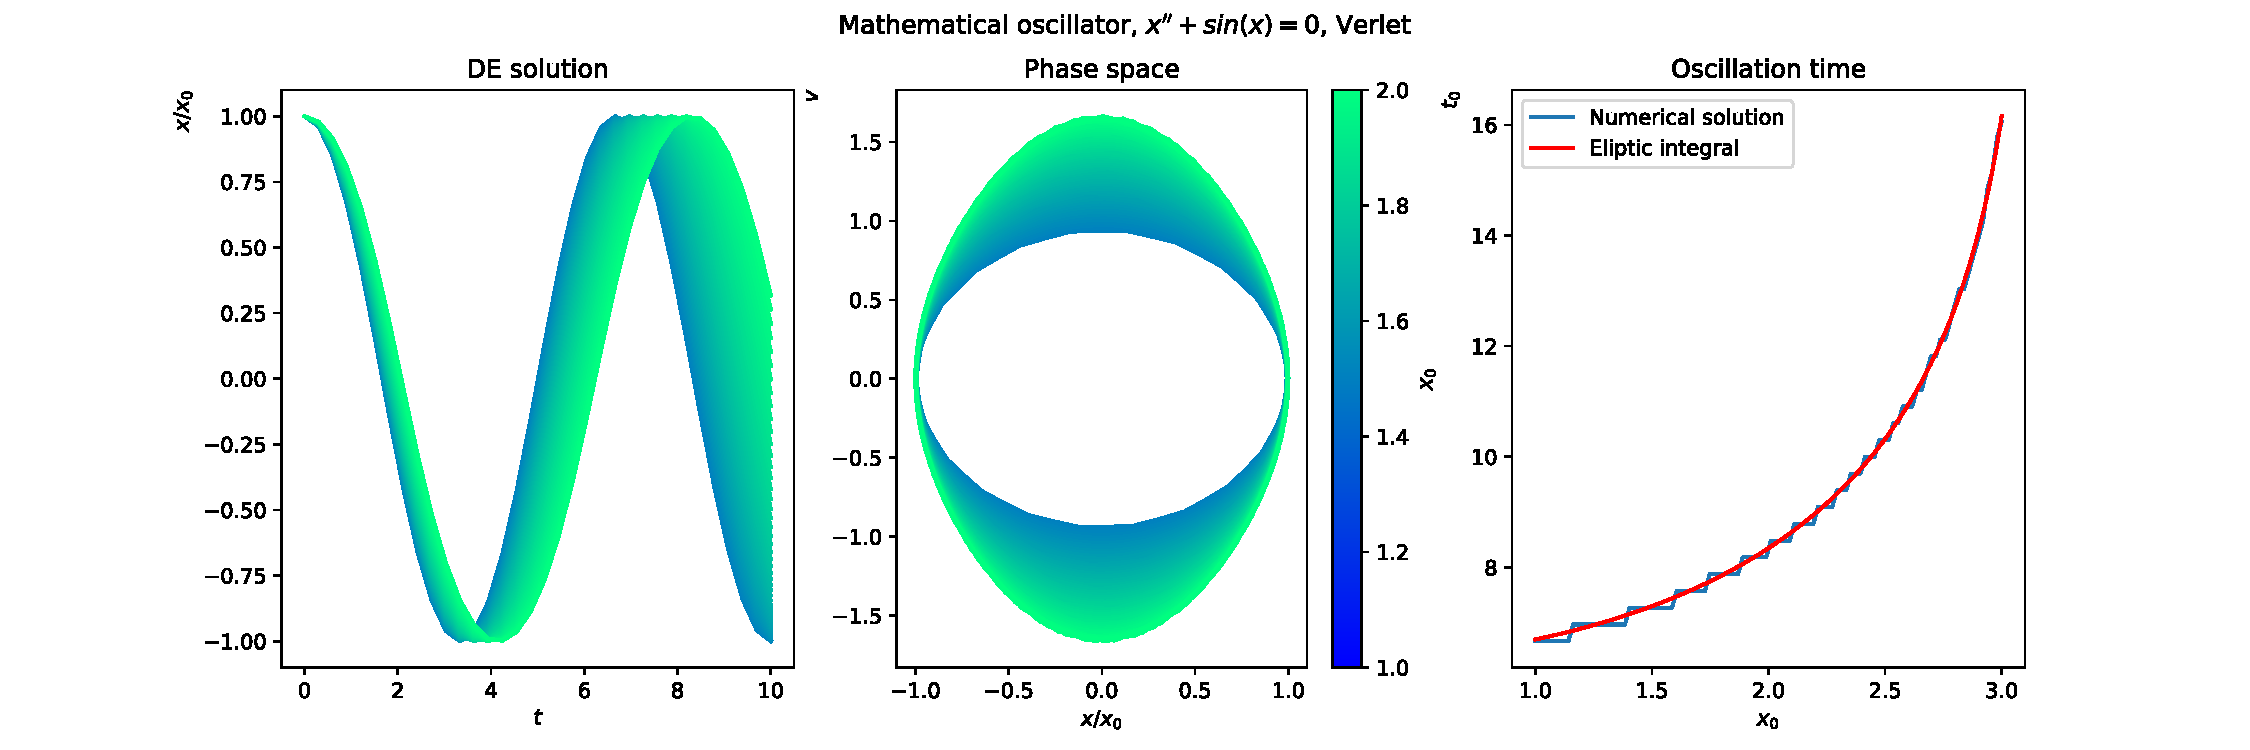
\includegraphics[width=15cm]{graphs/method_analysis.pdf}
  \end{center}
  \vspace*{-7mm}
  \caption{Analysis of mathematical oscillator.}
\end{figure}

The results above were computed using Verlet method, but let's compare it to other methods we might have used. We will differentiate between lower order methods (Euler, Heun, Midpont and Runge-Kutta 2) and higher order methods (Runge-Kutta 4, predictor-corrector, Runge-Kutta 45, Runge.Kutta-Fehlberg, Verlet and PEFRL).

The stability of a method is assessed by measuring the amplitude over time and by measuring the total error over time. Lower order methods tend to diverge from initial amplitude, the extreme here is the Euler method. Comparing these to high order methods we see that their error roughly stays the same. The spikes seen in Figure 2a are the result of numerics. Similar results can be concluded from Figure 2c.

As we are dealing with a non-dissipative system we want the energy to be conserved. Figure 2b shows the absolute error of energy compared to initial energy of the system. The energy stays constant only with symplectic methods (Verlet and PEFRL) in all other cases the total energy increases.

\begin{figure}[hbtp]
  \begin{center}
  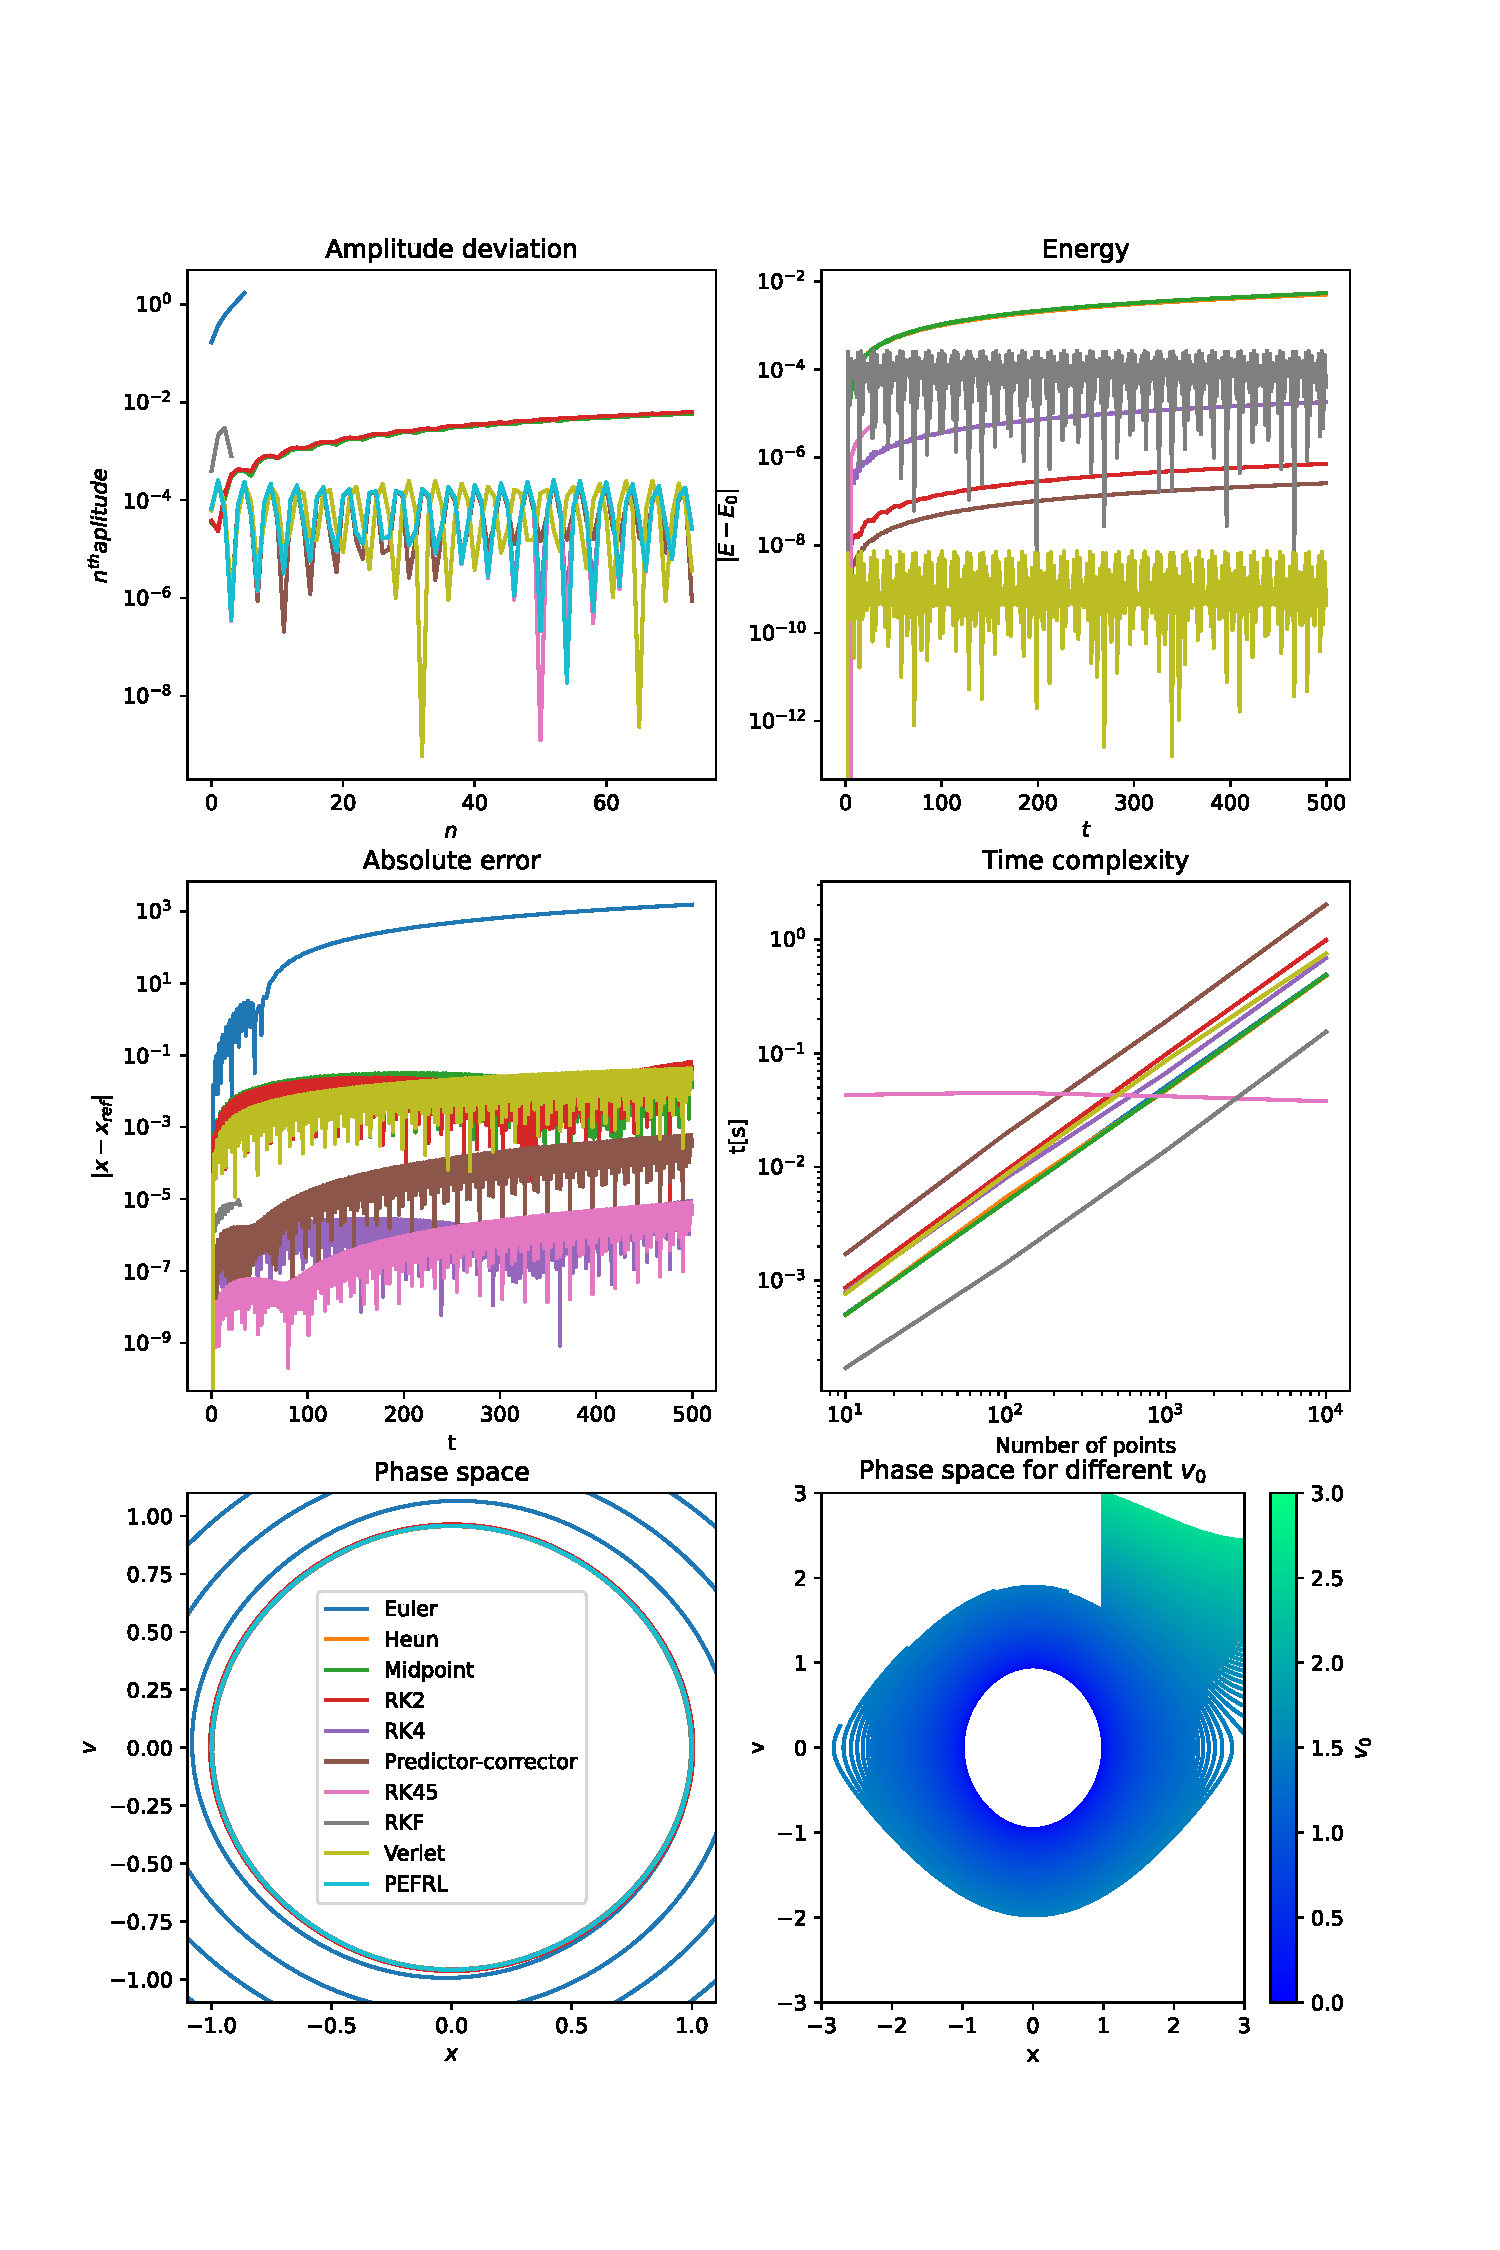
\includegraphics[width=14cm]{graphs/method_comparison.pdf}
  \end{center}
  \vspace*{-7mm}
  \caption{Analysis of numeric methods. The legend is the same for all of the graphs.}
\end{figure}

The third important factor is computation time and it’s dependence on number of points (step size). From Figure 2d we can conclude that computation time rises linearly. This relation comes from the use of one for loop. For a given step size we can see differences in computation times, which come from the time needed to perform one step of the algorithm. Therefore we can order the methods by speed in the following way going from fastest to slowest: RKF, Euler, Midpoint, Heun, RK4, Verlet, PEFRL, RK2, predictor-corrector. Computation time of RK45 is constant.

The phase space more visually shows us the deviation from initial energy. From Figure 2e we see how quickly the Euler method diverges. Some fluctuations can be seen with lower order methods, if we were to run the simulation longer these deviations would be more pronounced.

Lastly let's look at the phase space in comparison to different initial velocities, $x_0 = 1$. Imagine our problem as a ball oscillating in a sinusoidal potential. With low velocity the ball is able to stay in the first well of the potential (blue region), but if we increase this velocity the ball will have enough energy (green region) to get past the first well and into the second one. But because it is not losing any energy it still has enough speed to go over all the barriers. Both extreme cases and the transition between them can be seen on Figure 2e.

\begin{figure}[hbtp]
  \begin{center}
  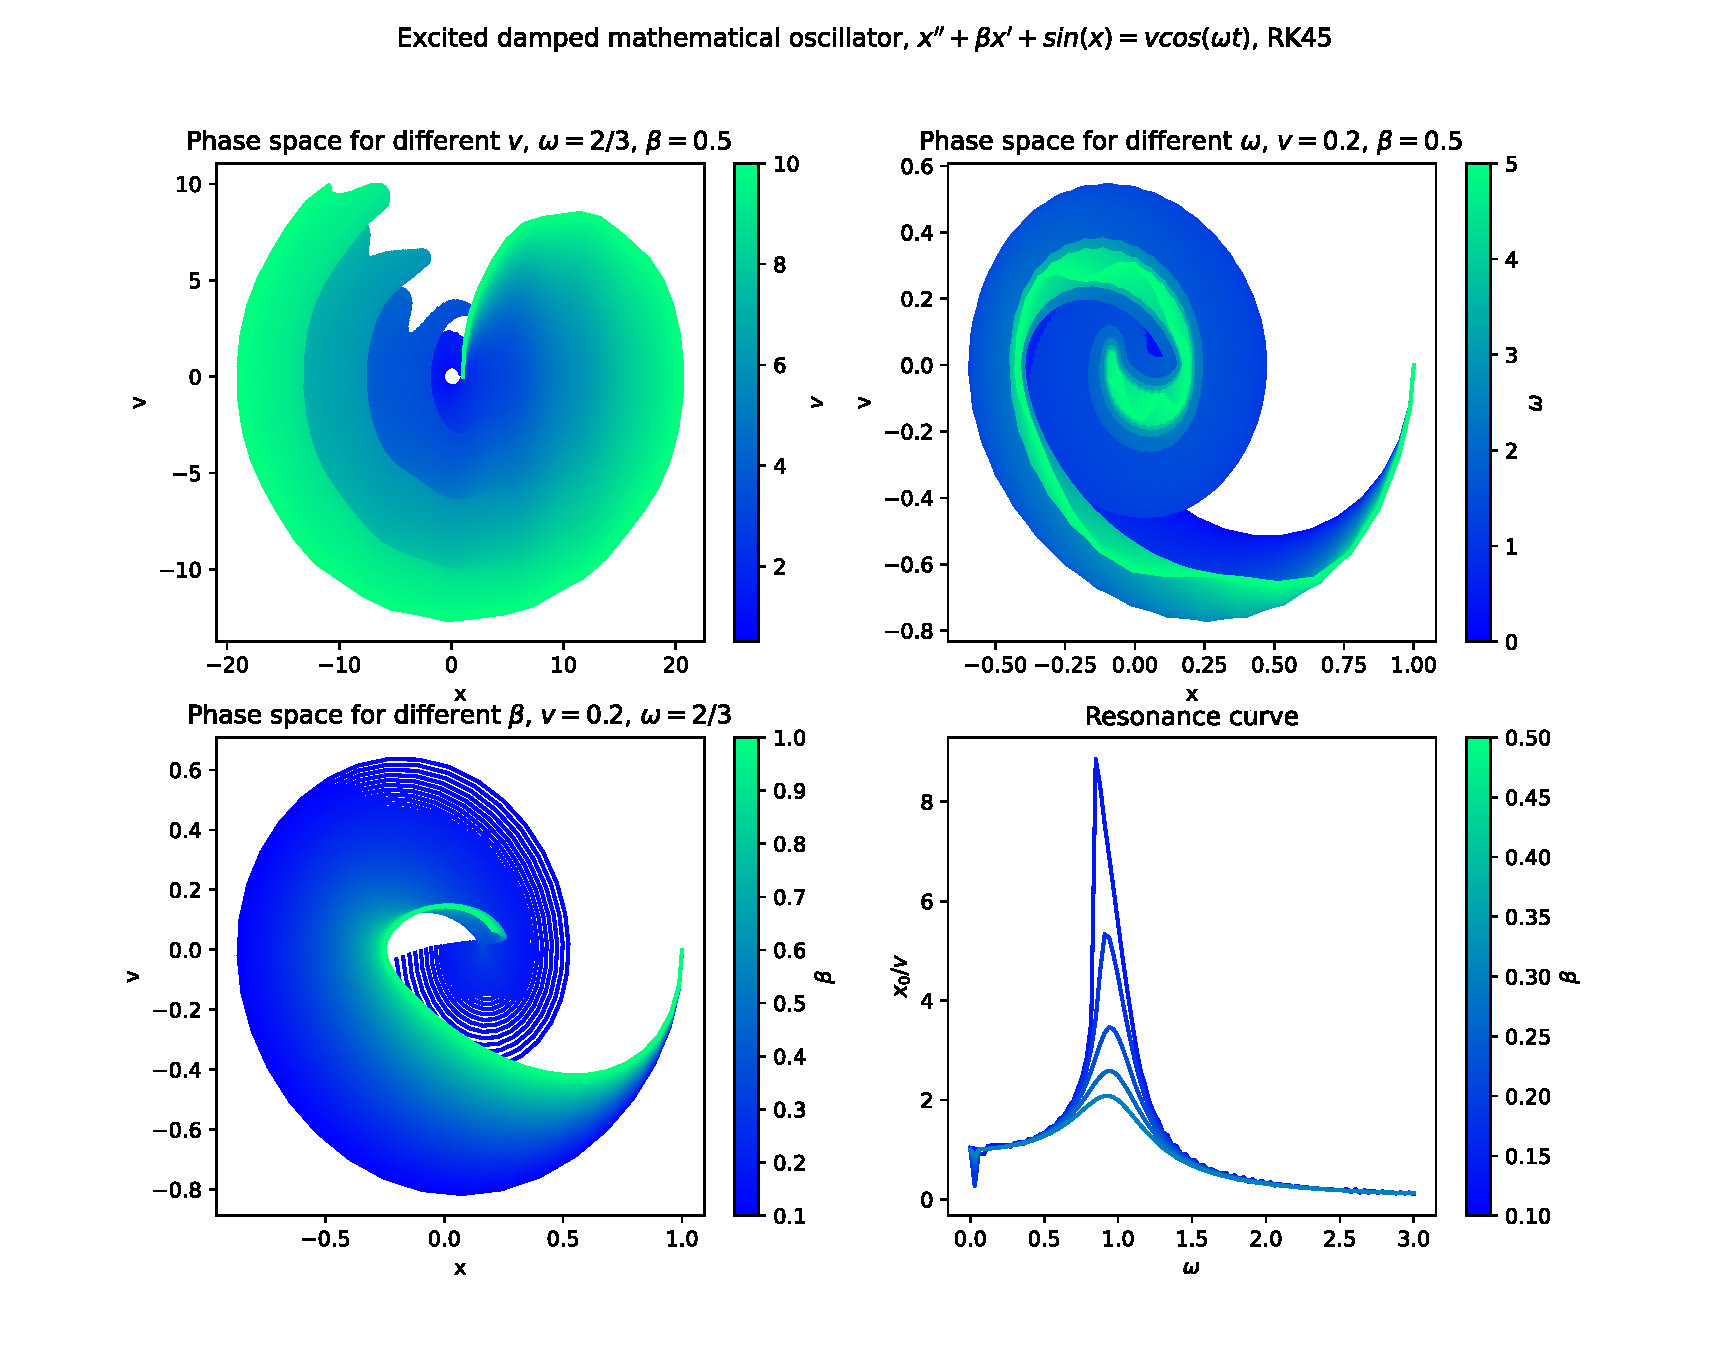
\includegraphics[width=15cm]{graphs/resonance2.pdf}
  \end{center}
  \vspace*{-7mm}
  \caption{Analysis of excited damped oscillator}
\end{figure}

\section{Excited damped mathematical oscillator} 

The second system we will analyse is a damped mathematical oscillator, which is described by three parameters: $\beta$ damping factor, $v$ excitation amplitude and $\omega$ excitation frequency.

By changing the amplitude of excitation we see that the oscillator amplitude quickly changes to that of the excitation. That's why we see almost concentric rings in Figure 3a. With time these rings would collapse to 0 due to the dampening factor.

Changing the dampening factor changes how quickly the oscillations die out. With higher $\beta$ we almost see critical dampening, where no oscillations occur.

The most interesting factor is the excitation frequency. The resonance frequency of our oscillator is 1. Figure 3b shows that higher frequencies (green region) quickly fade away, as the excitation is not helping the oscillator combat the damping force. The largest amplitudes can be observed around resonance frequencies (blue region). By looking how amplitude changes with respect to frequency and damping we get Figure 3d a resonance curve.

\section{Van der Pol oscillator}

Van der Pol oscillator is similar to previous one, the one big difference is that the damping factor is proportional to the square of the amplitude. This means the largest damping force will be at the extreme position of the oscillator. The system is defined by three parameters: $\omega$ and $v$, which are the same as previously and $\lambda$ the damping factor.

\begin{figure}[hbtp]
  \begin{center}
  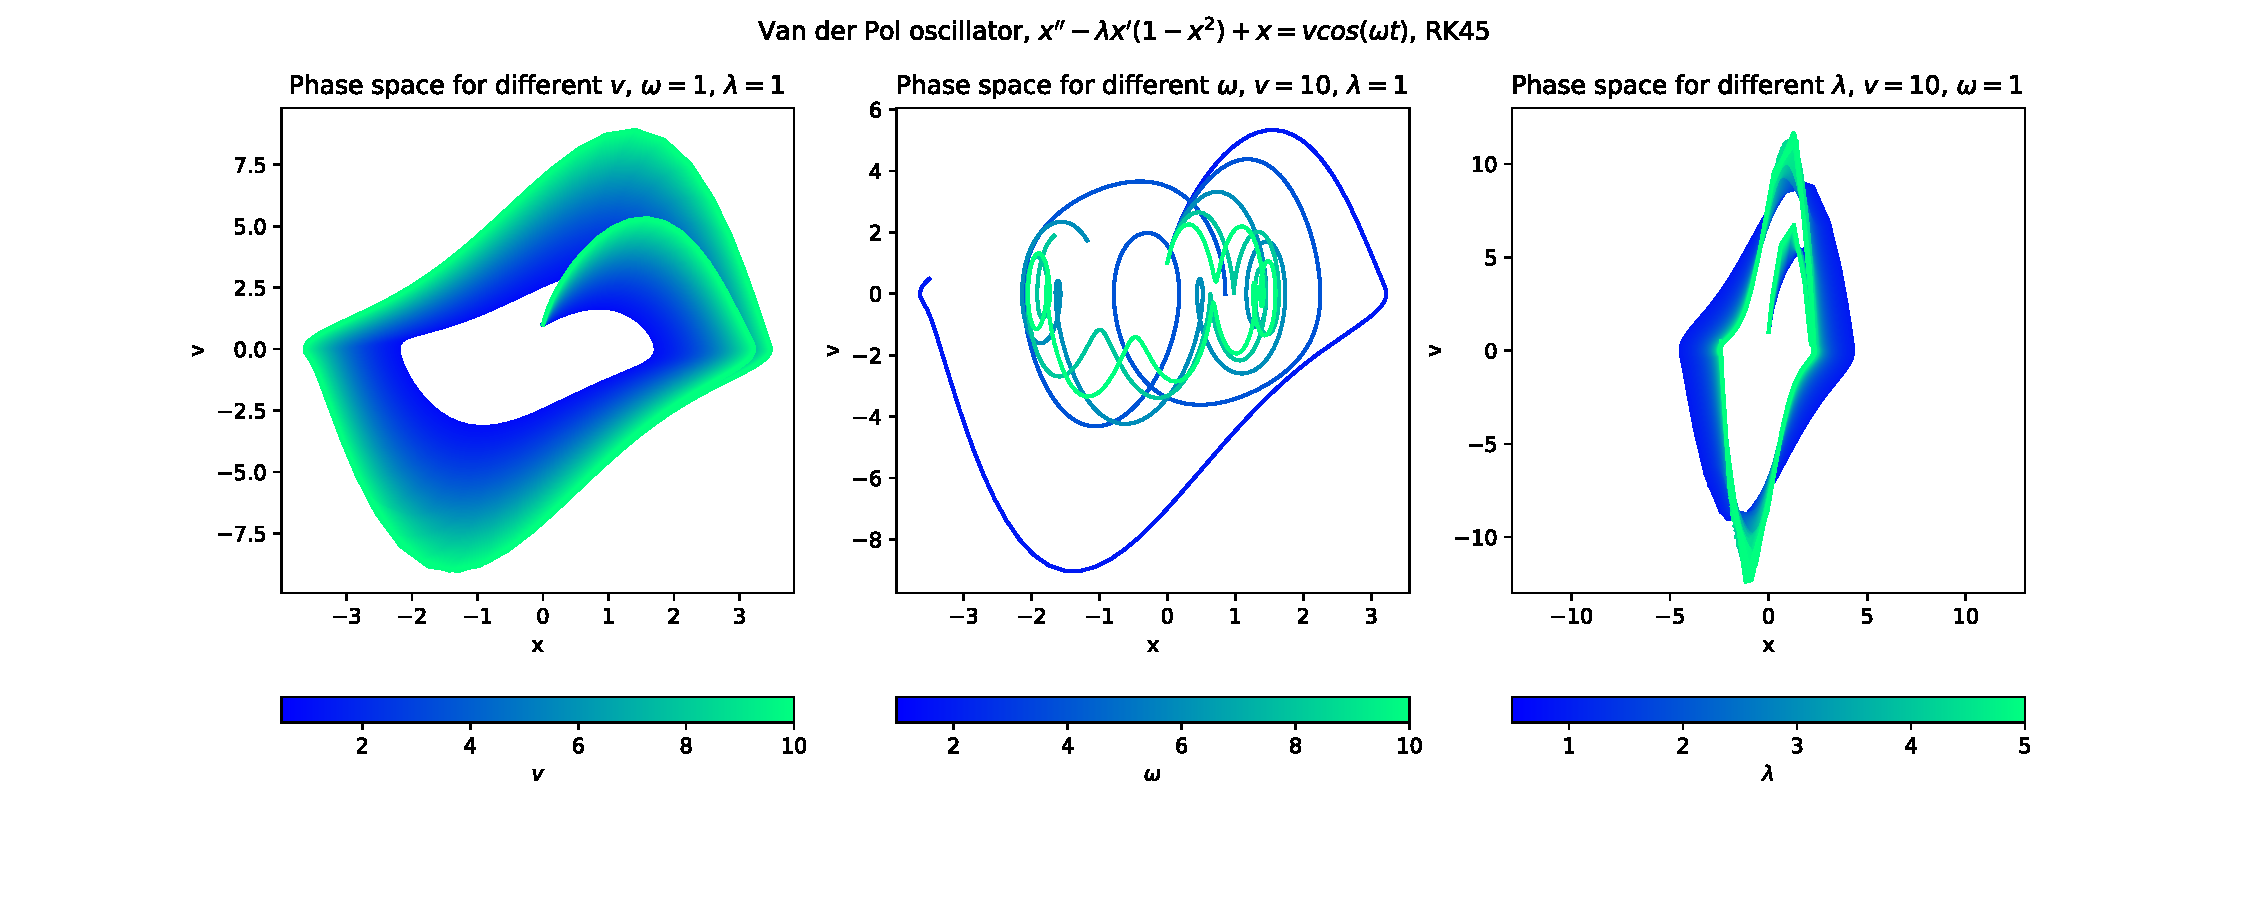
\includegraphics[width=15cm]{graphs/van_der_pol.pdf}
  \end{center}
  \vspace*{-7mm}
  \caption{Analysis of Van der Pol oscillator.}
\end{figure}

Let's analyse how these parameters affect the solution. The effect of $v$ is similar to previous oscillator, but what we can see is that as the oscillator starts moving away from the extreme position it's speed arises, as the damping force decreases. When we cross the equilibrium the force slowly increases and the oscillator starts slowing down. An increase in $\lambda$ (Figure 4c) will lower the amplitude and increase the speed, which is proportional to higher damping force. Figure 4b shows how the phase space changes with excitation frequency. At resonance frequency the amplitude is the highest, whereas with higher frequencies the movement becomes more chaotic and the amplitude drops.

\end{document}